\documentclass[a4paper, 12pt]{article}
\usepackage[margin=2cm]{geometry}
\usepackage{graphicx}
\usepackage[font=footnotesize]{caption}

\graphicspath{{Images}}

\author{BE19B009 - Shobhan Karthick}
\title{Assignment 2 \\ FitzHugh-Nagumo model}
\date{}

 \renewcommand{\familydefault}{\sfdefault}

\begin{document}  

\maketitle

\section{Introduction}
\label{Intro}

FitzHugh-Nagumo model is a simplifcation of the Hodgkin-Huxley model. The differential equation corresponding `m' and `j' are approximated to be constants and hence the model becomes a 2-variable model with the following equations.

$$ \frac{dV}{dt} = f(v) - w + I_m $$
$$ \frac{dw}{dt} = bv - rw $$
where, $ f(v) = v(a - v)(v - 1) $. Also, $ V_m, n $ from HH-model becomes the $ V, w $ variables in FN-model.

\section{Case 1: \boldmath{$ I_{ext} = 0 $}}
\label{case_1}
\subsection{Phase plot of v-nullcline and w-nullcline}

\begin{center}
    \begin{minipage}{\linewidth}
    \centering
    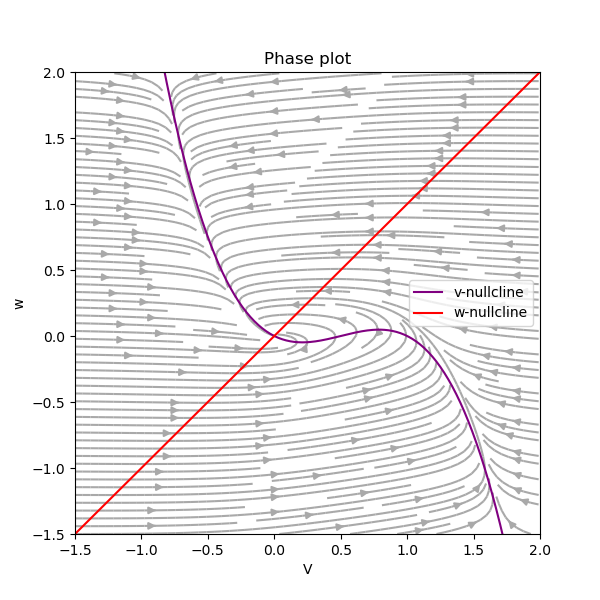
\includegraphics[width=0.55\textwidth]{Q1_a}
    \captionof{figure}{Super imposed phase plot v-nullcline and w-nullcline at $ I_{ext} = 0 $}
    \label{fig:Q1_a}
\end{minipage}
\end{center}

\noindent{
Phase plot as shown in Figure \ref{fig:Q1_a}, was plotted using stream plot from matplotlib library in Python. The grey arrows in plot depict the flow around the nullclines.
}

\subsection{Time plots for V(t) and W(t)}

Time plots for V(t) and W(t) are shown below for different conditions along with their phase plane trajectories.

\subsubsection{\boldmath{$ V(0) < 0; V(0) = 0.4; W(0) = 0 $}}

\begin{minipage}{0.48\linewidth}
    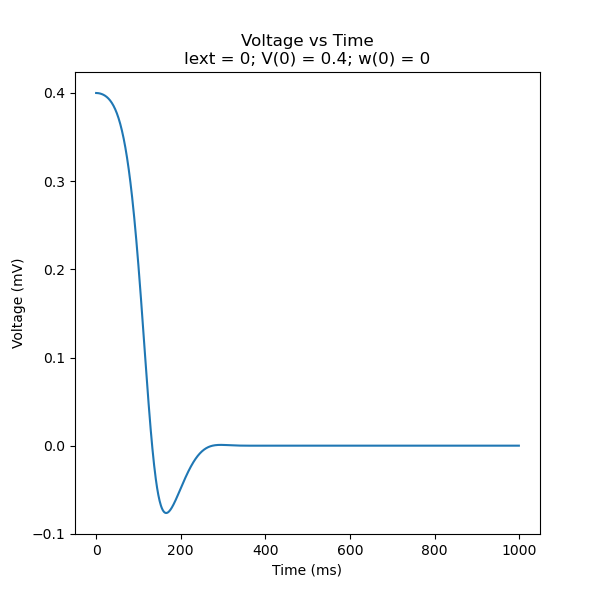
\includegraphics[width=\textwidth]{Q1_b_i_1}
    \captionof{figure}{V(t) vs t plot for $ I_{ext} = 0 $ with V(0) = 0.4}
    \label{fig:Q1_b_i_1}
\end{minipage}
\hfill
\begin{minipage}{0.48\linewidth}
    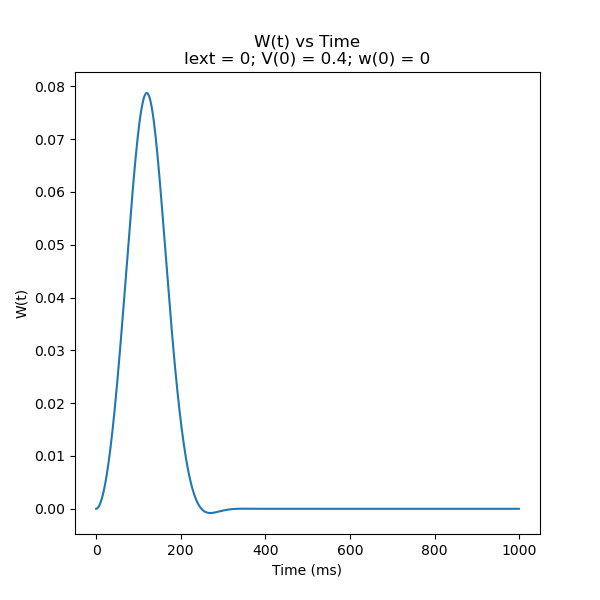
\includegraphics[width=\textwidth]{Q1_b_i_2}
    \captionof{figure}{W(t) vs t plot for $ I_{ext} = 0 $ with V(0) = 0.4}
    \label{fig:Q1_b_i_2}
\end{minipage}

\begin{minipage}{\linewidth}
    \centering
    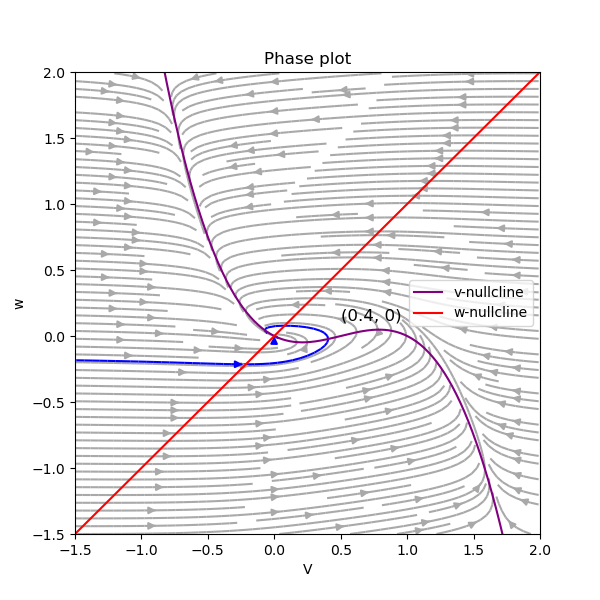
\includegraphics[width=0.7\textwidth]{Q1_b_i_3}
    \captionof{figure}{Phase plot of the trajectory of V(0) = 0.4 \& W(0) = 0}
    \label{fig:Q1_b_i_3}
\end{minipage}

\subsubsection{\boldmath{$ V(0) < 0; V(0) = 0.4; W(0) = 0 $}}

\begin{minipage}[t]{0.48\linewidth}
    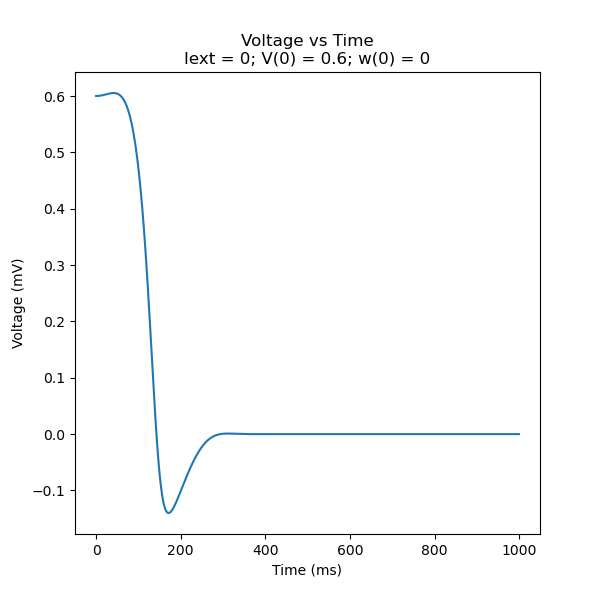
\includegraphics[width=\textwidth]{Q1_b_ii_1}
    \captionof{figure}{V(t) vs t plot for $ I_{ext} = 0 $ with V(0) = 0.6}
    \label{fig:Q2_b_i_1}
\end{minipage}
\hfill
\begin{minipage}[t]{0.48\linewidth}
    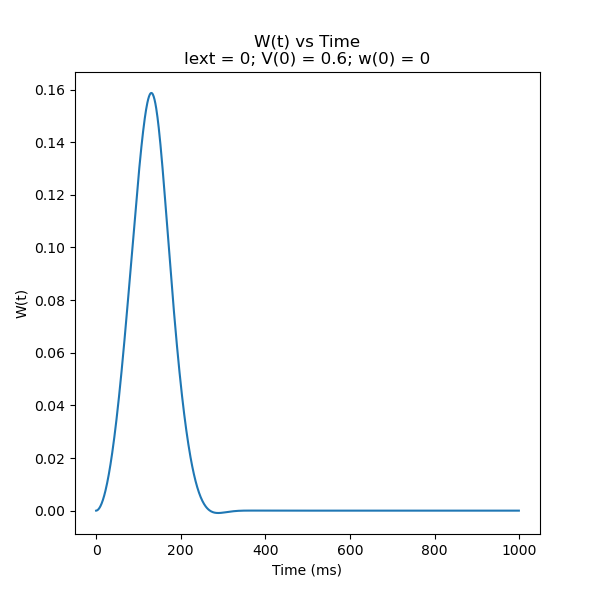
\includegraphics[width=\textwidth]{Q1_b_ii_2}
    \captionof{figure}{W(t) vs t plot for $ I_{ext} = 0 $ with V(0) = 0.6}
    \label{fig:Q2_b_i_2}
\end{minipage}


\begin{minipage}{\linewidth}
    \centering
    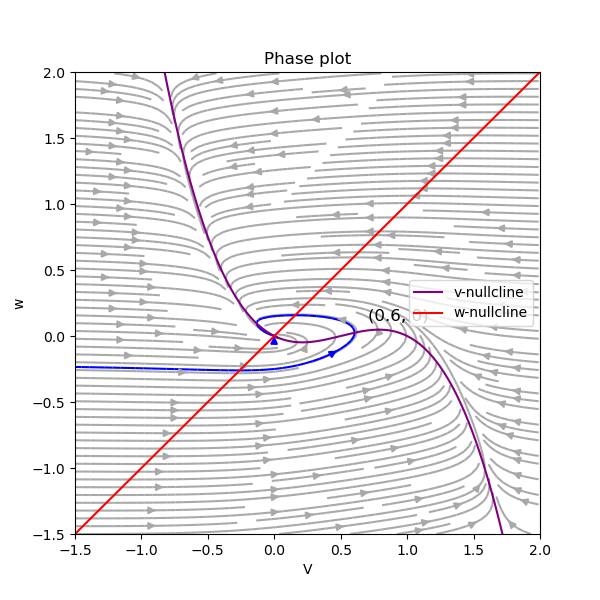
\includegraphics[width=0.7\textwidth]{Q1_b_ii_3}
    \captionof{figure}{Phase plot of the trajectory of V(0) = 0.6 \& W(0) = 0}
    \label{fig:Q2_b_i_3}
\end{minipage}

\section{Case 2: \boldmath{$ I_1 < I_{ext} < I_2 $}}
\label{case_2}

In order to find $ I_1 $ \& $ I_2 $, the $ I_{ext} $ was varied such that after $ I_1 $, there were oscillations and after $ I_2 $ there are no oscillations. So, $ I_1 $ came out to be 0.23 and $ I_2 $ came out to be 0.80.

\subsection{\boldmath{$ I_1~ \& ~I_2 $} plots; V(0) $ < $ a; V(0) = 4;}

\begin{minipage}{0.45\linewidth}
    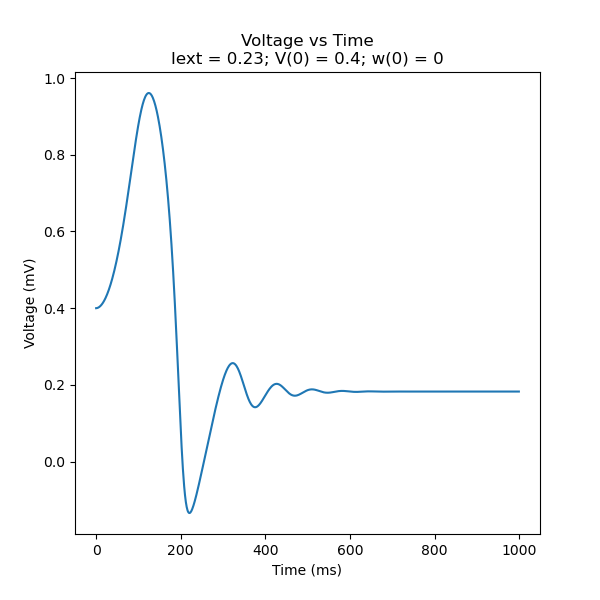
\includegraphics[width=\textwidth]{Q2_1}
    \captionof{figure}{V(t) vs t at $ I_{ext} = 0.23 $}
    \label{fig:Q2_1}
\end{minipage}
\hfill
\begin{minipage}{0.45\linewidth}
    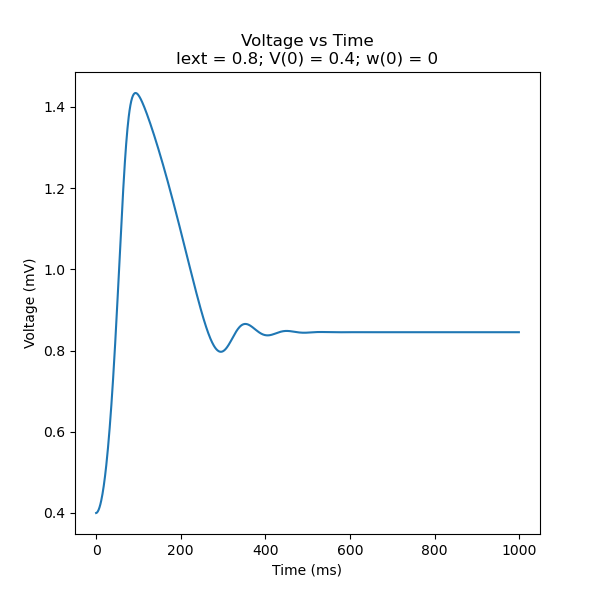
\includegraphics[width=\textwidth]{Q2_5}
    \captionof{figure}{V(t) vs t at $ I_{ext} = 0.80 $}
    \label{fig:Q2_5}
\end{minipage}

\vspace{2em}
\noindent
The figures \ref{fig:Q2_1} and \ref{fig:Q2_5} shows the plots at $ I_1 = 0.23 mV ~ \& ~ I_2 = 0.80 mV$ respectively at the V(0) = 0.4 mV. So after 0.23 mV, there will oscillations and after 0.80 mV, there will be no oscillations at all.

\subsection{\boldmath{$ I_1~ \& ~I_2 $} plots; V(0) $ < $ a; V(0) = 4;}

\begin{minipage}{0.45\linewidth}
    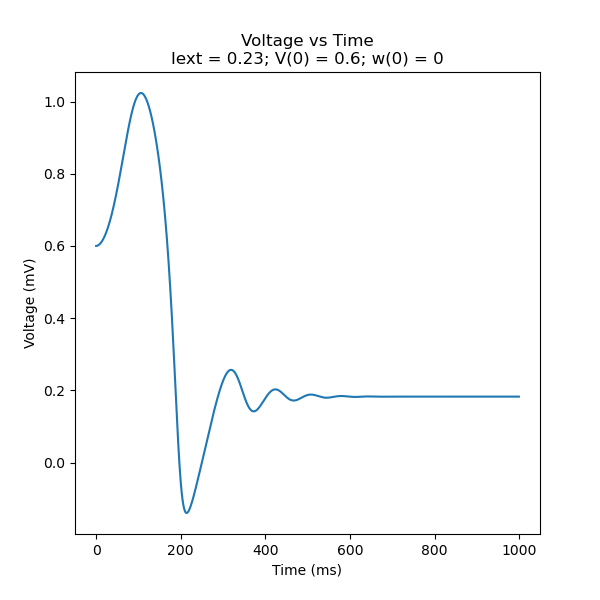
\includegraphics[width=\textwidth]{Q2_3}
    \captionof{figure}{V(t) vs t at $ I_{ext} = 0.23 $}
    \label{fig:Q2_3}
\end{minipage}
\hfill
\begin{minipage}{0.45\linewidth}
    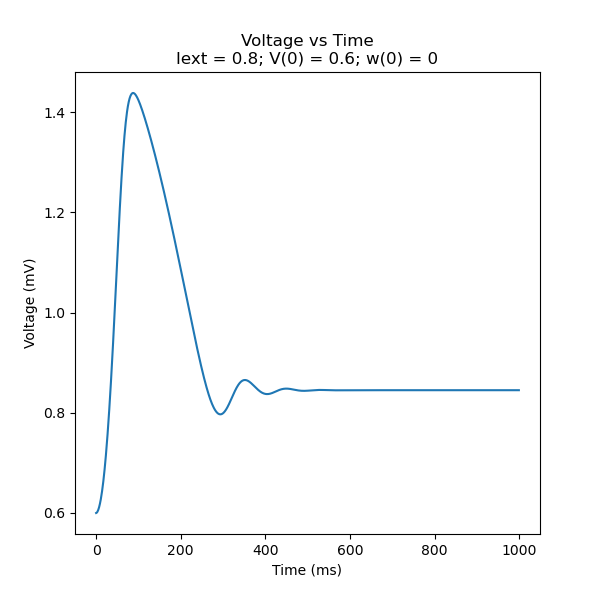
\includegraphics[width=\textwidth]{Q2_7}
    \captionof{figure}{V(t) vs t at $ I_{ext} = 0.80 $}
    \label{fig:Q2_7}
\end{minipage}

\vspace{2em}
\noindent
The figures \ref{fig:Q2_3} and \ref{fig:Q2_7} shows the plots at $ I_1 = 0.23 mV ~ \& ~ I_2 = 0.80 mV$ respectively at the V(0) = 0.6 mV. So after 0.23 mV, there will oscillations and after 0.80 mV, there will be no oscillations at all.

\subsection{Phase plot for \boldmath{$ I_{ext} = 0.5 $}}

\begin{minipage}{0.48\linewidth}
    \centering
    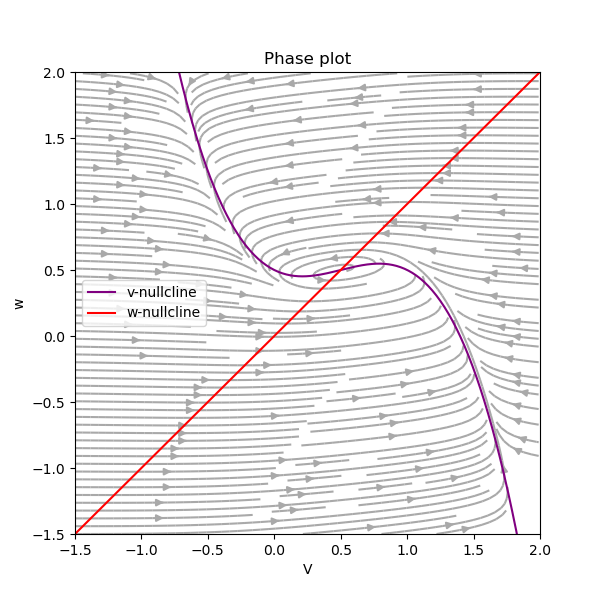
\includegraphics[width=\textwidth]{Q2_a}
    \captionof{figure}{Phase plot of $ I_{ext} = 0.5 $}
    \label{fig:Q2_a}
\end{minipage}
\hfill
\begin{minipage}{0.48\linewidth}
    \centering
    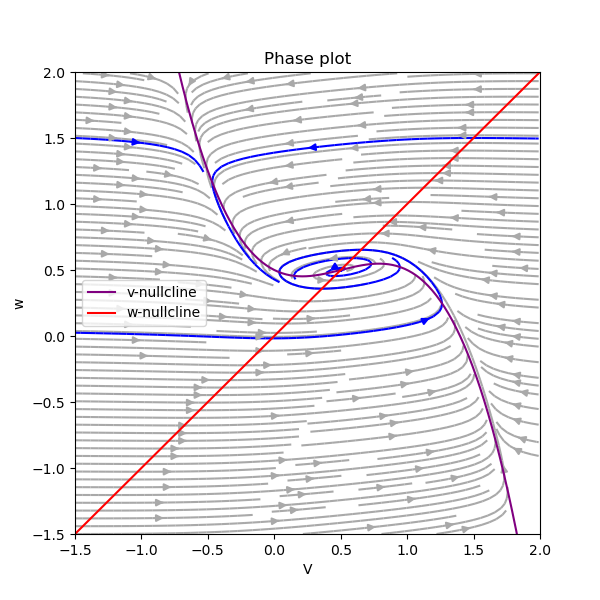
\includegraphics[width=\textwidth]{Q2_b_1}
    \captionof{figure}{Trajectories showing the fixed point produces stable limit cycle}
    \label{fig:Q2_b_1}
\end{minipage}

\vspace{2em}
As shown in figure \ref{fig:Q2_b_1}, there is a stable limit cycle which is produced by the unstable node at (0.5, 0.5). From wherever you start, either from inside the limit cycle i.e. very close to the unstable node or from outside i.e. totally away from the nullclines, the trajectory follows and comes into the limit cycle.

\subsection{Time plots for V(t) and W(t) for \boldmath{$ I_{ext} = 0.5 $} }

Time plots for V(t) and W(t) are shown below for different conditions at an $ I_{ext} = 0.5 $ 

\subsubsection{\boldmath{$ V(0) < 0; V(0) = 0.4; W(0) = 0 $}}

\begin{minipage}[t]{0.48\linewidth}
    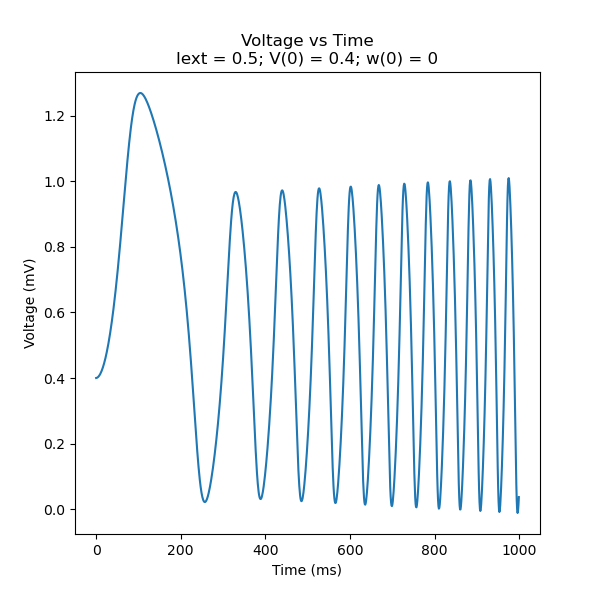
\includegraphics[width=\textwidth]{Q2_c_1}
    \captionof{figure}{V(t) vs t plot for $ I_{ext} = 0.5 $ with V(0) = 0.4}
    \label{fig:Q2_c_1}
\end{minipage}
\hfill
\begin{minipage}[t]{0.48\linewidth}
    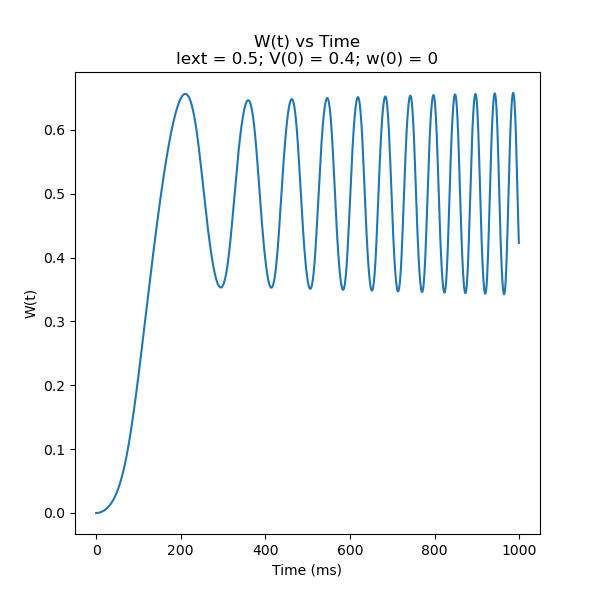
\includegraphics[width=\textwidth]{Q2_c_2}
    \captionof{figure}{W(t) vs t plot for $ I_{ext} = 0.5 $ with V(0) = 0.6}
    \label{fig:Q2_c_2}
\end{minipage}

\subsubsection{\boldmath{$ V(0) > 0; V(0) = 0.6; W(0) = 0 $}}

\begin{minipage}[t]{0.48\linewidth}
    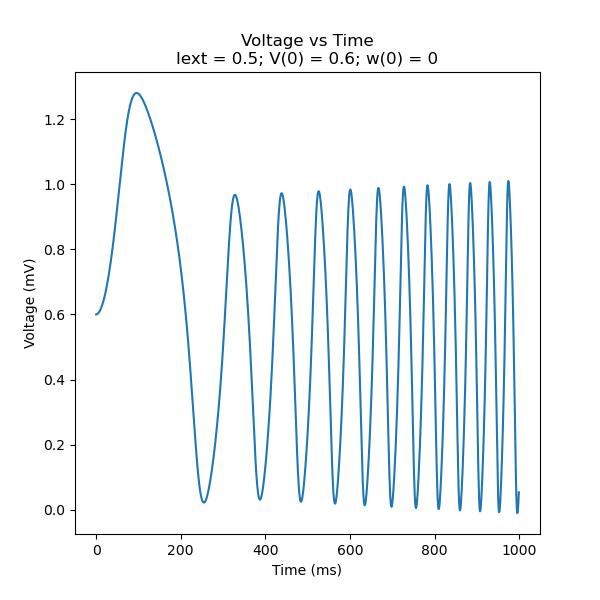
\includegraphics[width=\textwidth]{Q2_c_3}
    \captionof{figure}{V(t) vs t plot for $ I_{ext} = 0.5 $ with V(0) = 0.6}
    \label{fig:Q2_c_3}
\end{minipage}
\hfill
\begin{minipage}[t]{0.48\linewidth}
    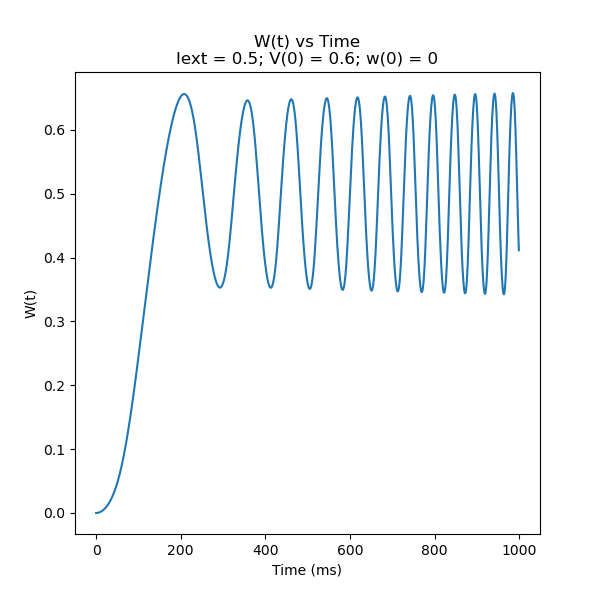
\includegraphics[width=\textwidth]{Q2_c_4}
    \captionof{figure}{W(t) vs t plot for $ I_{ext} = 0.5 $ with V(0) = 0.6}
    \label{fig:Q2_c_4}
\end{minipage}

\vspace{2em}
\noindent
For both initial values, V(0) = 0.4 and V(0) = 0.6 there are a lot of oscillations. W(t) vs t plots for both the inital value of $ V $ as shown in figures \ref{fig:Q2_c_2} and \ref{fig:Q2_c_4} look very alike.

\section{Case 3: \boldmath{$ I_{ext} > I_2 $}}
\label{case_3}

\subsection{Phase plot for \boldmath{$ I_{ext} = 0.5 $}}

\begin{minipage}{0.48\linewidth}
    \centering
    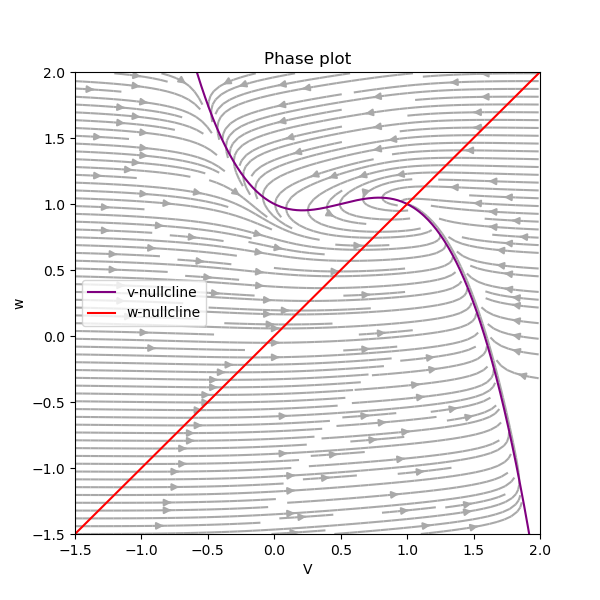
\includegraphics[width=\textwidth]{Q3_a}
    \captionof{figure}{Phase plot of $ I_{ext} = 1.0 $}
    \label{fig:Q3_a}
\end{minipage}
\hfill
\begin{minipage}{0.48\linewidth}
    \centering
    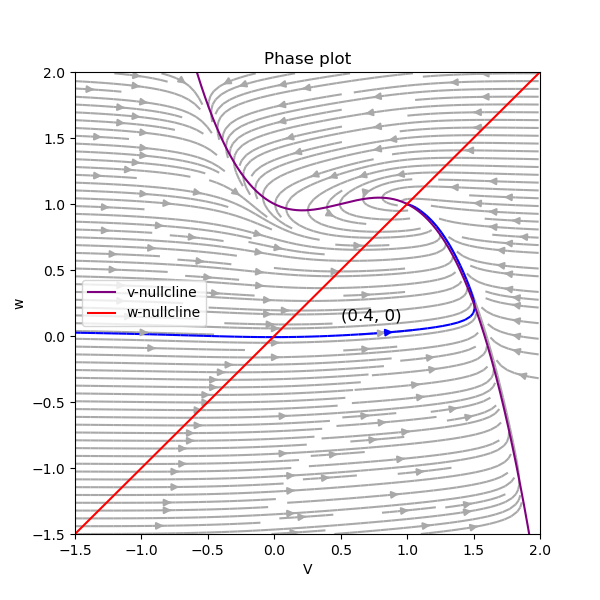
\includegraphics[width=\textwidth]{Q3_b}
    \captionof{figure}{Trajectories showing the fixed point produces unstable limit cycle}
    \label{fig:Q3_b}
\end{minipage}

\vspace{2em}
\subsection{Time plots for V(t) and W(t) for \boldmath{$ I_{ext} = 1.0 $} }

Time plots for V(t) and W(t) are shown below for different conditions at an $ I_{ext} = 1.0 $ 

\subsubsection{\boldmath{$ V(0) < 0; V(0) = 0.4; W(0) = 0 $}}

\begin{minipage}[t]{0.48\linewidth}
    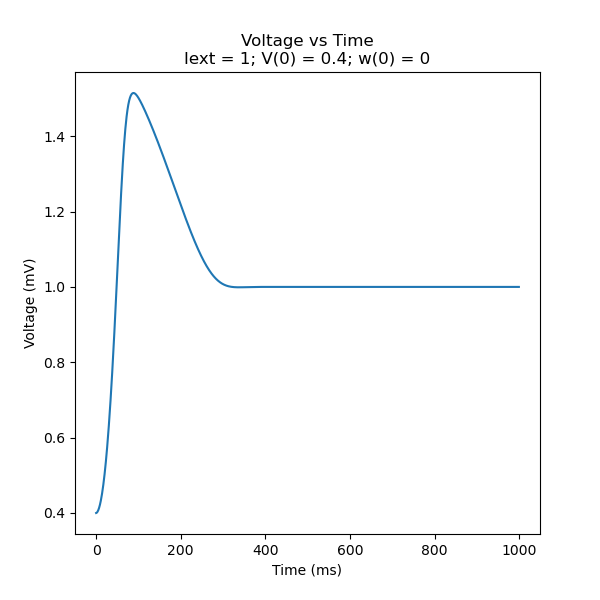
\includegraphics[width=\textwidth]{Q3_c_1}
    \captionof{figure}{V(t) vs t plot for $ I_{ext} = 1.0 $ with V(0) = 0.4}
    \label{fig:Q3_c_1}
\end{minipage}
\hfill
\begin{minipage}[t]{0.48\linewidth}
    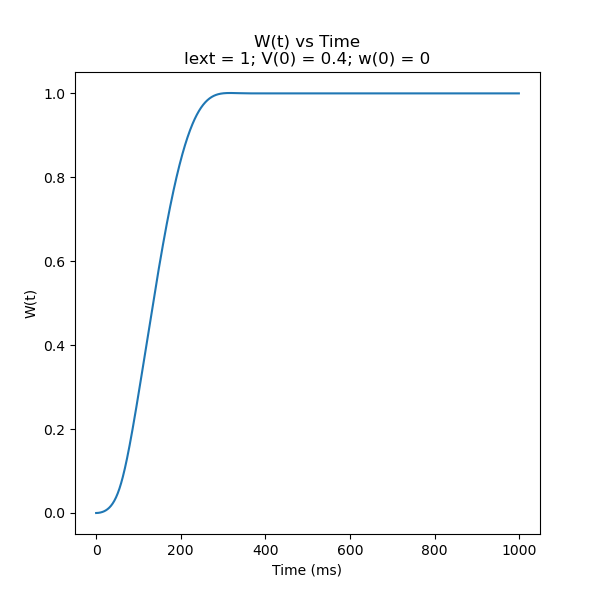
\includegraphics[width=\textwidth]{Q3_c_2}
    \captionof{figure}{W(t) vs t plot for $ I_{ext} = 1.0 $ with V(0) = 0.6}
    \label{fig:Q3_c_2}
\end{minipage}

\subsubsection{\boldmath{$ V(0) > 0; V(0) = 0.6; W(0) = 0 $}}

\begin{minipage}[t]{0.48\linewidth}
    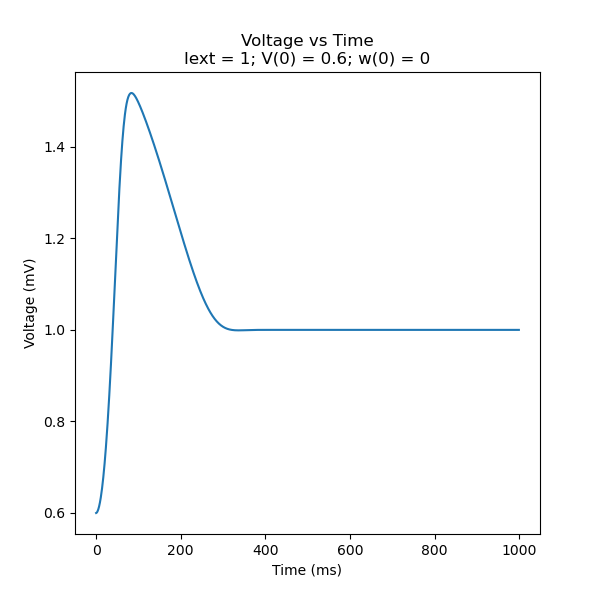
\includegraphics[width=\textwidth]{Q3_c_3}
    \captionof{figure}{V(t) vs t plot for $ I_{ext} = 1.0 $ with V(0) = 0.6}
    \label{fig:Q3_c_3}
\end{minipage}
\hfill
\begin{minipage}[t]{0.48\linewidth}
    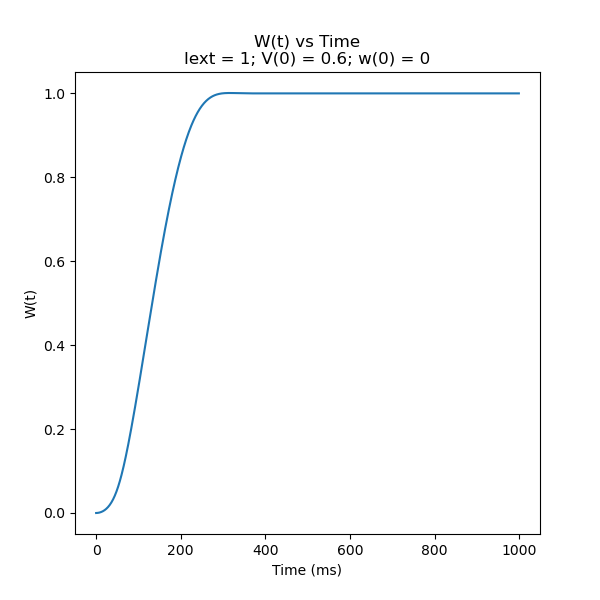
\includegraphics[width=\textwidth]{Q3_c_4}
    \captionof{figure}{W(t) vs t plot for $ I_{ext} = 1.0 $ with V(0) = 0.6}
    \label{fig:Q3_c_4}
\end{minipage}

\vspace{2em}
\noindent


\section{Case 4: \boldmath{$ I_{ext} = 0;~ \frac{b}{r} = 0;$}}
\label{case_4}

\subsection{Bistability Phase plot}

\begin{minipage}{\linewidth}
    \centering
    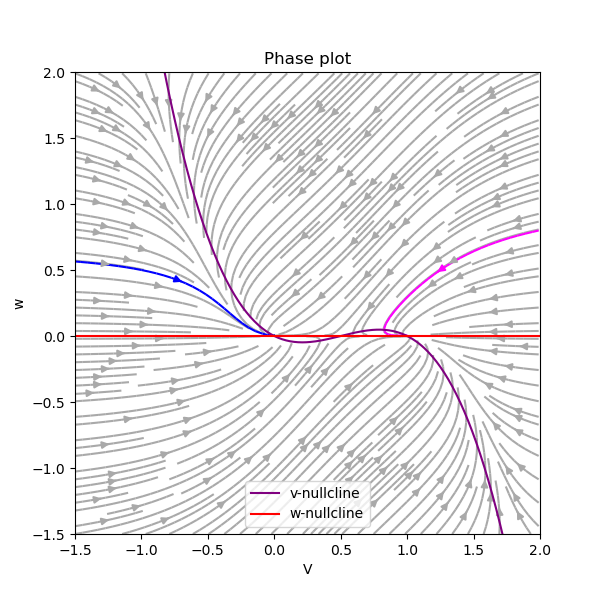
\includegraphics[width=0.60\textwidth]{Q4_a}
    \captionof{figure}{Phase plot of $ I_{ext} = 0; ~ \frac{b}{r} = 0; $}
    \label{fig:Q4_a}
\end{minipage}

\subsection{Time plots for V(t) and W(t) for \boldmath{$ I_{ext} = 0 ~ \& ~ \frac{b}{r} = 0 $} }
Time plots for V(t) and W(t) are shown below for different conditions at an $ I_{ext} = 0 ~ \& ~ \frac{b}{r} = 0 $ 

\subsubsection{\boldmath{$ V(0) < 0; V(0) = 0.4; W(0) = 0 $}}

\begin{minipage}[t]{0.48\linewidth}
    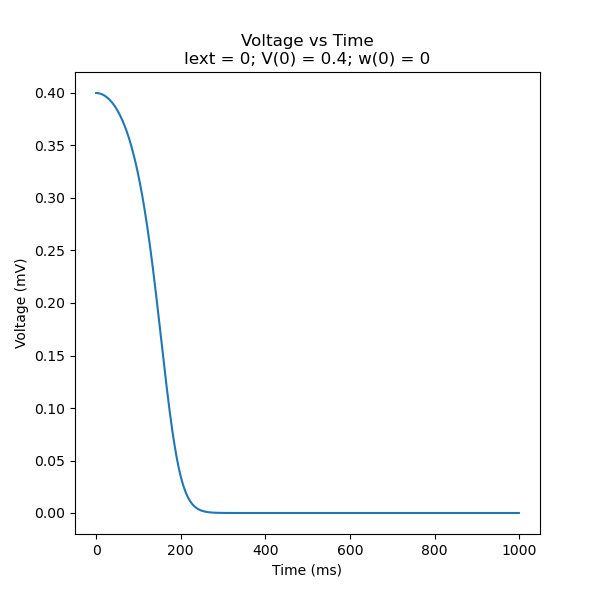
\includegraphics[width=\textwidth]{Q4_c_1}
    \captionof{figure}{V(t) vs t plot for $ I_{ext} = 1.0 $ with V(0) = 0.4}
    \label{fig:Q4_c_1}
\end{minipage}
\hfill
\begin{minipage}[t]{0.48\linewidth}
    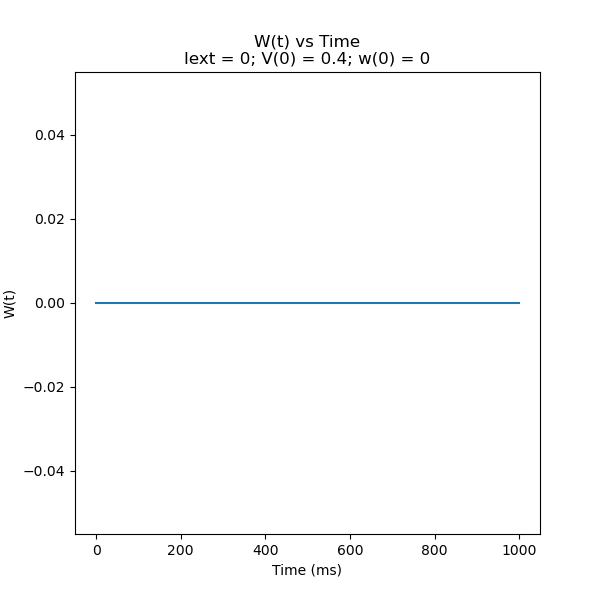
\includegraphics[width=\textwidth]{Q4_c_2}
    \captionof{figure}{W(t) vs t plot for $ I_{ext} = 1.0 $ with V(0) = 0.6}
    \label{fig:Q4_c_2}
\end{minipage}

\subsubsection{\boldmath{$ V(0) > 0; V(0) = 0.6; W(0) = 0 $}}

\begin{minipage}[t]{0.48\linewidth}
    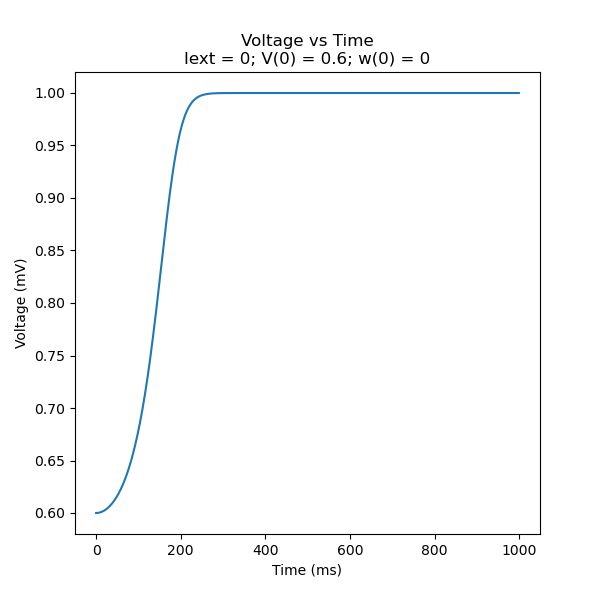
\includegraphics[width=\textwidth]{Q4_c_3}
    \captionof{figure}{V(t) vs t plot for $ I_{ext} = 1.0 $ with V(0) = 0.6}
    \label{fig:Q4_c_3}
\end{minipage}
\hfill
\begin{minipage}[t]{0.48\linewidth}
    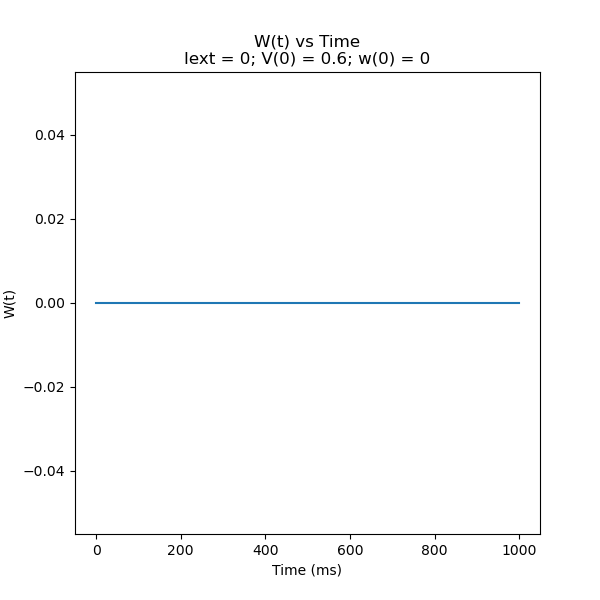
\includegraphics[width=\textwidth]{Q4_c_4}
    \captionof{figure}{W(t) vs t plot for $ I_{ext} = 1.0 $ with V(0) = 0.6}
    \label{fig:Q4_c_4}
\end{minipage}

\vspace{2em}
From figure \ref{fig:Q4_a}, Let P1, P2, P3 be the points of intersection of the W nullcline and V nullcline from
left to right. For P1, a small perturbation will bring back the point to P1. Hence, P1 is
stable. This is the same case with P3 too. Since there are 2 stable points, this condition is called as bistability.

\noindent
In the case of P2, any perturbation will result in moving away from P2 and it will move into one of the stable fixed points.

\end{document}
